\chapter{Modelos de Inversão Sísmica}
\label{cap:2modelosInversao}


Numa configuração de experimentos físicos se tem o espaço dos parâmetros do
modelo e o espaço das medidas. No contexto da sísmica de reflexão, os dados
sísmicos $d$ são representados no espaço das medidas e a propriedade de
impedância acústica $m$ das rochas é representada no espaço do modelo.

A princípio parece descomplicada a utilização de equações físicas que descrevem
o sistema de forma inversa, fazendo o mapeamento do espaço das medidas ao espaço
do modelo. No entanto, esses métodos de inversão direta sofrem de instabilidades
devido à ruído e características do problema \citep[p. 50]{sen_livro}. Outra
opção é utilizar tentativa e erro para ajustar os parâmetros até conseguir uma
resposta semelhante aos dados experimentais. Formalmente isto é automatizado
utilizando métodos de otimização. Para tanto, é preciso definir uma função de
custo, ou função objetivo, que mede o ajuste dos dados produzidos pelos
parâmetros do modelo (dado sintético) ao dado medido.

O objetivo da inversão, no entanto, vai além de encontrar os parâmetros que
melhor se ajustam aos dados. Quando os dados são ruidosos, o modelo direto não é
exato e não existem dados suficientes, a inversão tem solução não única, ou
seja, vários modelos ajustam aos dados de forma equivalente. Consequentemente é
importante modelar a incerteza envolvida no processo, indicando qual a
variabilidade dos modelos que se ajustam bem aos dados.

A relação entre o modelo e os dados (modelo direto) é dada por:

\begin{equation}
d = G(m_v) + e
\end{equation}
onde $G(\cdot)$ é uma função não linear, e assume-se que um ruído $e$ está
presente. Em teoria o ruído é uma interferência aleatória que não se tem
controle, na prática se considera ruído tudo que não é explicado pela função
$G$, e.g. imprecisões no modelo físico e problemas com filtragem e processamento
dos dados.

\section{Inversão Sísmica Linear e Não Linear}

O modelo mais utilizado para aproximar a função $G$, no caso da inversão
sísmica, é o modelo convolucional. No caso discreto a convolução é dada pelo
produto acumulado de cada amostra do vetor de refletividades por todas as
amostras da \textit{wavelet}. Portanto pode ser representado por uma operação
matricial:

\begin{equation}
\label{eq:sismDiscreta}
\mathbf{d = Gr}
\end{equation}
onde $\mathbf{G}$ é uma matriz convolucional construída utilizando uma
\textit{wavelet} e $\mathbf r$ o vetor das refletividades definido por:

\begin{equation}
\label{eq:refletDiscreta}
r(t)=\frac{z(t+\delta t) - z(t)}{z(t+\delta t) + z(t)}
\end{equation}
o que torna não linear a relação entre impedância $\mathbf z$ e o dado sísmico.
Uma aproximação válida quando valores de refletividades não ultrapassam $0.3$ é:


\begin{equation}
r(t) = \frac{1}{2}\Delta \ln(z(t))
\label{eq:lnz}
\end{equation}


Utilizando estas aproximações para o modelo direto, a alternativa mais objetiva
é incorporar as aproximações na matriz $\mathbf{G}$ e invertê-la para obter
$\mathbf{\ln(z)}$, por fim aplicar o exponencial para obter $\mathbf{z}$.
Neste caso temos os seguintes problemas: existência; unicidade; estabilidade; e
robustez \citep[p. 56-57]{sen_livro}. Utilizando a formulação de mínimos
quadrados também é possível resolver sistemas sobredeterminados, solucionando
problemas com a melhor estimativa possível no sentido de minimizar o erro
quadrático (norma $L_2$). Apesar de ser uma solução mais geral, ainda é
utilizado somente um critério de ajuste aos dados, o que não possibilita a
inserção de conhecimento \textit{a priori}. É possível regularizar o método de
mínimos quadrados, mas ainda não se tem muita liberdade para inserir
conhecimentos \textit{a priori} e de outras fontes \citep{clappRegLeast3D}.


Quando não é possível o uso da aproximação da Equação \ref{eq:lnz}, o problema
deve ser abordado utilizando métodos de otimização não linear. Com isso os erros
devido às aproximações do modelo \textit{forward} diminuem, mas a otimização se
torna mais custosa. Como a relação entre os dados e os parâmetros é não linear, a
função objetivo a ser minimizada irá possuir mínimos locais, tornando necessário
o uso de métodos de otimização global. Esta prática está bem documentada na
literatura de inversão, como o uso de \textit{simulated annealing}
\citep{max_inv_simulated}, de algoritmos genéticos \citep{MallickGeneticInve} e
enxame de partículas \citep{zhe_nonlinear}. 


%falar mais das vantagens e desvantagens do nao linear

Outra forma de inversão presente na literatura é a elástica
\citep{azevedo2013_avoinv,Buland01012003}. Nesse tipo de inversão os dados
sísmicos estão em um nível diferente de processamento onde os traços sísmicos
são empilhados em intervalos de ângulos de incidência. Com isso é possível
inverter para Vp (velocidade primária/compressional), Vs (velocidade
secundária/cisalhante) e $\rho$ (densidade), ao invés de somente impedância
acústica. A Equação \ref{eq:elastica} modela a relação da refletividade $c_{pp}$
com Vp ($\alpha$), Vs ($\beta$) e $\rho$ para cada ângulo disponível.

\begin{equation}
c_{pp}(\theta) = a_\alpha(\theta)\frac{\Delta\alpha}{\bar{\alpha}} +
a_\beta(\theta) \frac{\Delta\beta}{\bar{\beta}} +
a_\rho(\theta) \frac{\Delta\rho}{\bar{\rho}}
\label{eq:elastica}
\end{equation}

onde:
\begin{equation}
a_\alpha(\theta)= \frac{1}{2}(1+\tan^2\theta),
\end{equation}

\begin{equation}
a_\beta(\theta)= -4\frac{\bar{\beta}^2}{\bar{\alpha}^2}\sin^2\theta,
\end{equation}

\begin{equation}
a_\rho(\theta) = \frac{1}{2} \left (  
1-4\frac{\bar{\beta}^2}{\bar{\alpha}^2}\sin^2\theta \right ).
\end{equation}

Adicionalmente $\bar{\alpha}$, $\bar{\beta}$ e $\bar{\rho}$ são as respectivas
médias sobre a interface; $\Delta\alpha$, $\Delta\beta$ e $\Delta\rho$ são os
contrastes e $\theta$ o ângulo médio de reflexão. Essas propriedades são
importantes, pois a velocidade secundária é indicador de hidrocarbonetos por não
se propagar em meio líquido, desta forma áreas com presença destes compostos se
destacam numa imagem de Vs, podendo indicar interfaces rocha/óleo e água/óleo.
As metodologias para resolução do problema são semelhantes, mas neste caso
aumentando a dimensão dos dados e números de parâmetros a serem estimados
\citep{Buland01012003}.

\subsection{Máximo \textit{a posteriori}}
\label{sec:map}

A inversão por Máximo \textit{a posteriori} (MAP)
\citep{Buland01012003,leandroGRSL} é realizada para cada traço individualmente.
Baseado no modelo convolucional e assumindo que o ruído presente nos dados é
Gaussiano, o vetor das sísmicas experimentais $\boldsymbol{d}$, é modelado pela
distribuição de probabilidade:

\begin{equation}
p(\boldsymbol{d}|\boldsymbol{\mu_{d}},\boldsymbol{\Sigma_{d}}) =
N(\boldsymbol{\mu_{d}},\boldsymbol{\Sigma_{d}}),
\end{equation}
onde $\boldsymbol{\mu_{d}} = \boldsymbol{Gm}$ é o vetor com a sísmica
sintética e $\boldsymbol{\Sigma_{d}}$ é a matriz de covariância do ruído da
sísmica, a qual é definida conforme a confiabilidade que o especialista tem no
dado sísmico ou seu nível de ruído. Geralmente se utiliza uma matriz diagonal
com mesma variância para todos os elementos.

Para o vetor modelo $\boldsymbol{m}$ com o logaritmo natural da impedância
acústica, considerou-se também uma distribuição normal:

\begin{equation}
p(\boldsymbol{m}|\boldsymbol{\mu_{m}},\boldsymbol{\Sigma_{m}}) =
N(\boldsymbol{\mu_{m}},\boldsymbol{\Sigma_{m}}),
\end{equation} 
no qual $\boldsymbol{\mu_{m}}$ é um vetor contendo a baixa frequência do
logaritmo natural da impedância. Este dado é outra informação adicional que é
fornecida pelo especialista via análise de velocidades ou interpolando
dados de poços por Krigagem. Os componentes da matriz de covariância
$\boldsymbol{\Sigma_{m}}$ foram definidos conforme \citep{leandroGRSL}:

\begin{equation}
\label{eq:correlVert}
\boldsymbol{\nu}_{t,t'} = \sigma_{m}^{2} exp \left (-\frac{(t-t')^2)}{L^2}
\right ),
\end{equation} 
que define a correlação entre as componentes de $\boldsymbol{m}$ no tempo $t$ e
$t'$, na qual $\sigma_{m}^{2}$ é a variância da impedância acústica calculada
nos dados de poços sem a baixa frequência, e $L$ é a distância de correlação
vertical a ser imposta ao resultado.

Neste arcabouço a média e variância posterior para cada traço podem ser
calculadas analiticamente via \citep{leandroGRSL}:

\begin{equation}
\label{eqn:mapSolution}
\boldsymbol{\mu}_{m|} = \boldsymbol{\mu}_{m} + \boldsymbol{\Sigma}_{m}\boldsymbol{G}^{T}(\boldsymbol{G\Sigma}_{m}\boldsymbol{G}^{T}+\boldsymbol{\Sigma}_{d})^{-1}\left ( \boldsymbol{d}_{o} - \boldsymbol{G\mu}_{m} \right ),
\end{equation}
\begin{equation}
\boldsymbol{\Sigma}_{m|} = \boldsymbol{\Sigma}_{m} - \boldsymbol{\Sigma}_{m}\boldsymbol{G}^{T}(\boldsymbol{G\Sigma}_{m}\boldsymbol{G}^{T}+\boldsymbol{\Sigma}_{d})^{-1}\boldsymbol{G\Sigma}_{m}.
\end{equation} 
onde o cálculo da matriz inversa acima pode ser aproveitado para vários traços
de uma região de interesse em certos casos, ou seja, quando as matrizes de
covariância possam ser assumidas iguais para todos os traços da sísmica da região.
Desta forma alteram-se a sísmica $\mathbf{d}_0$ e a baixa frequência
$\boldsymbol{\mu_m}$ obtendo-se a média posterior para o traço desejado.


Utilizando esta metodologia a solução é representada por uma distribuição
posterior Gaussiana com expressões explícitas para o valor esperado e para a
covariância. Não são necessárias iterações para ajuste do modelo, tornando o
método eficiente e útil em casos de uso reais, possibilitando o especialista
alterar parâmetros e avaliar o resultado em tempo real numa pequena área.
Satisfeito com a parametrização, o método é aplicado a todo o campo. A matriz de
covariância posterior indica a incerteza presente no resultado, não é necessário
definir a tolerância de ajuste aos dados explicitamente, mas é preciso definir a
matriz de covariância \textit{a priori} do resultado esperado, ou seja, é
preciso ter conhecimento, mesmo que de forma grosseira, das correlações espaciais e
variâncias que se espera do resultado. Ao final, a covariância posterior é
calculada.

Uma desvantagem destacada na literatura é a dificuldade em inserir modelos de
continuidade mais abrangentes, pois é necessário incluir as covariâncias entre
traços vizinhos, aumentando as matrizes de covariância e a matriz a ser
invertida. Inserindo as correlações horizontais também inviabiliza aproveitar o
cálculo da matriz inversa, pois desta forma o resultado da inversão precisa ser
calculado para todos os pontos a serem invertidos ao mesmo tempo.
Atualmente é inserida somente covariância entre amostras no mesmo traço, ou
seja, somente na direção vertical.

\section{Modelagem de Incerteza}

Novas propostas surgiram recentemente para tentar encontrar modelos
$\mathbf{m}_f \in \mathbf{M} \subset \mathbf{R}^N$, onde $\mathbf M$ é o
conjunto de modelos admissíveis que atendem o conhecimento \textit{a priori} e
são consistentes com o domínio do problema \citep{TompkinsScalabUnce2011}. Para o
problema da incerteza, o objetivo é encontrar o conjunto de modelos pertencentes
a $\mathbf M$ que se ajustam aos dados observados com uma certa tolerância
($tol$):

\begin{equation}
||G\mathbf{(m)-d}||_p \leq tol
\end{equation}
onde $||\cdot||_p$ é uma norma $L_p$ de erro escolhida. Na prática esse
parâmetro cria um vale plano na função de erro  \citep{Martinez2011Topogra}, como
ilustrado em uma dimensão na Figura \ref{fig:erroFunc}.

\begin{figure}[htp]
\begin{center}
  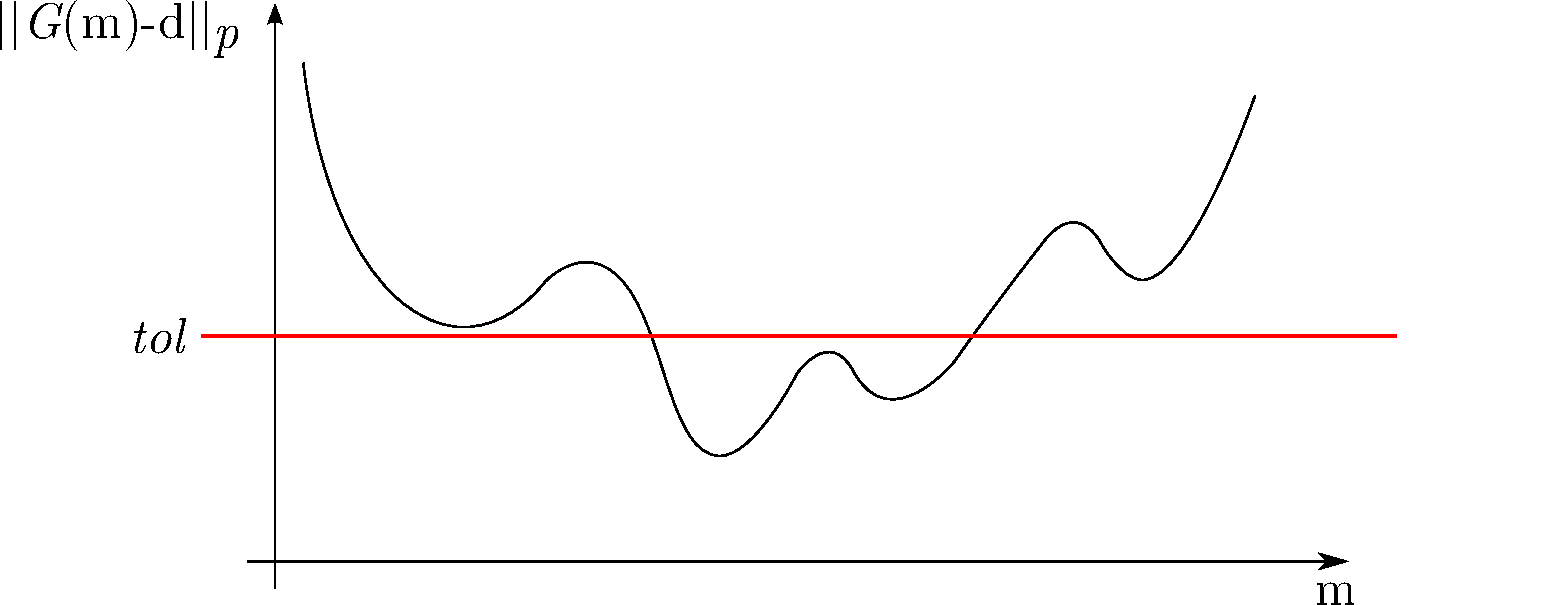
\includegraphics[width=0.7\textwidth]{fig/errorFuncTol}
  \caption{Efeito da tolerância na função de erro}
  \label{fig:erroFunc}
\end{center}
\end{figure}

A justificativa para o uso desse nível de tolerância é evitar o ajuste dos dados
ao ruído. No caso do erro atingir o mínimo, o modelo está tentando explicar o
ruído presente nos dados medidos. Apesar da Figura \ref{fig:erroFunc} ser uma
simplificação, consegue-se perceber que ao adicionar a tolerância um conjunto de
modelos passa a ser aceitável. Sem a tolerância um só modelo seria eleito como
melhor e não teríamos a estimativa da incerteza, apesar de se ajustar melhor aos
dados. Este parâmetro é definido empiricamente e deve refletir a incerteza e o
ruído presente nos dados.

Na técnica MAP, citada anteriormente na Seção \ref{sec:map}, além de retornar a
matriz de covariância indicando a incerteza presente no resultado, não é
necessário definir a tolerância explicitamente, mas é preciso definir a matriz
de covariância \textit{a priori} do resultado esperado, ou seja, é preciso ter
conhecimento, mesmo que de forma grosseira, das correlações espaciais e
variâncias que se espera do resultado. Ao final, a covariância posterior é
calculada e o conhecimento \textit{a priori} é atualizado com os dados. Uma
desvantagem importante é a dificuldade em inserir modelos de continuidade mais abrangentes,
pois para tanto é necessário incluir as covariâncias entre os pontos a serem
estimados. Atualmente é inserida somente covariância entre amostras no mesmo
traço, ou seja, somente na direção vertical. Inserir covariância em outras
direções aumenta o número de elementos da matriz de covariância de forma
quadrática, tornando o processo custoso.

Utilizando uma abordagem estocástica Bayesiana, \cite{leandro_SEG} leva em
consideração a incerteza na \textit{wavelet} gerando amostras das distribuições
posteriores da impedância acústica e da \textit{wavelet}. O problema continua
linearizado e com suposição Gaussiana, mas é preciso utilizar um esquema de
amostragem baseado em simulação \textit{Markov-chain Monte Carlo} (MCMC) via
algoritmo de Gibbs, pois não é possível obter as distribuições posteriores
analiticamente. Com realizações da distribuição posterior, é possível calcular
as estatísticas de interesse e modelar a incerteza envolvida. A desvantagem é o
alto custo computacional para gerar amostras dessas distribuições,
principalmente com o aumento da dimensão do problema. Um estudo recente utiliza
MCMC para realizar amostragem da propriedades de porosidade e permeabilidade das
rochas \citep{zunino2014}. Estas propriedades são geralmente estimadas em uma
etapa posterior à estimativa de propriedades primárias, como a impedância.
Portanto o método gera interesse ao realizar inversão de forma mais avançada no
fluxo de trabalho, além de gerar estimativas da incerteza. Apesar de sofrer com
o alto custo computacional da amostragem o autor relata bons resultados.

A estimativa de \textit{wavelets} também é objeto de estudo na literatura. O
problema consiste em determinar o pulso sísmico que gerou o sinal medido,
utilizando os dados de poços como referência. \textit{Wavelets} podem ser
consideradas o elo entre os dados sísmicos e as propriedades de rocha. Como
podem haver erros de conversão da escala de profundidade dos poços para a escala
de tempo dos dados sísmicos, é necessário avaliar a incerteza na estimativa da
\textit{wavelet}. Por isso, um esquema de amostragem semelhante, baseado em 
MCMC, foi utilizado em \cite{BulandWavStochastic}.

Esforços na área de inteligência computacional foram inicialmente empregados
utilizando métodos que possuem componentes estocásticas, mas foram desenvolvidos
originalmente para explotação, ou seja, encontrar rapidamente o mínimo global da
função objetivo \citep{Sen1995v}. Otimização por enxame de partículas é um
exemplo. O método foi modificado para permanecer em sua fase de exploração,
favorecendo soluções que ficam abaixo de certa tolerância. Realizando, portanto,
o que é chamado de \textit{importance sampling} \citep{Martinez:2010PSO}. Os
autores dessa metodologia defendem que a função de erro é um bom \textit{proxy}
para a distribuição posterior.

Trabalhos anteriores tentaram sem êxito utilizar várias execuções de algoritmos
genéticos (GA) para estimar a incerteza \citep[p. 152]{Sen1995v}. A hipótese de
trabalho era a que ao executar o algoritmo várias vezes, seriam encontrados
vários mínimos locais que representariam a incerteza. Mas como demonstrado em
\cite{Martinez2011Topogra}, a topografia da função de erro em inversão sísmica
possui grandes vales alongados de mínimo global. Com isso os métodos devem ser
modificados para capturar essa característica e portanto, a simples execução
múltipla não gera boa estimativa da incerteza.

O trabalho de \cite{TompkinsScalabUnce2011} trata de inversão de dados
eletromagnéticos, outro tipo de metodologia utilizada na indústria para
imageamento de subsuperfície. Neste problema o modelo direto é mais complexo e
não linear. Apesar de não utilizar dados sísmicos, a metodologia proposta tem
objetivos pertinentes a inversão sísmica. A hipótese é que não é necessário
amostrar exaustivamente a distribuição posterior para modelar a incerteza, e sim
utilizar amostras representativas. A proposta utiliza redução dimensional
com análise de componentes principais (PCA) sobre a matriz de covariância.
Esta matriz, por sua vez, é calculada a partir de um conjunto de soluções ou
aproximada utilizando informação do gradiente da função objetivo após a execução
de um método de inversão não linear. Restrições \textit{a priori} são mapeadas
para o espaço reduzido e a técnica de \cite{smolyak63quadrature} é utilizada para
amostrar de forma determinística e hierárquica este espaço. Retornando ao espaço
original, é utilizado um critério de rejeição para eliminar soluções acima de
certa tolerância. Os passos de amostragem e rejeição são repetidos, refinando o
\textit{grid} de Smolyak, até que haja convergência de estatísticas das amostras
aceitas.

Ao reduzir a dimensão do problema se perde resolução espacial das amostras a
serem geradas, pois serão considerados somente parte dos primeiros autovetores,
ordenados de forma decrescente em relação aos seus autovalores, da matriz de
covariância. Ou seja, menores variabilidades são desconsideradas \citep[p.
3]{jolliffe2002principal}. Essa perda é justificada por serem desprezíveis em
certos casos e pela diminuição do custo computacional ao trabalhar no espaço
reduzido. Além do custo de computar os autovetores e autovalores, são
adicionados os custos de computar o grid de Smolyak e do mapeamento de
restrições do espaço original ao espaço reduzido. Esses custos extras se tornam
proibitivos quando a dimensão do problema cresce e não é mais possível reduzir a
dimensão à centenas de variáveis. Com isso alternativas surgiram para tentar
expandir o limite do tamanho do problema, em detrimento da resolução das
amostras utilizando decomposição em valores singulares
\citep{TompkinsScalabUnce2011} e utilizando outro esquema de amostragem
determinística \citep{TompkinsCupature}. Apesar dos avanços não se sabe se é
possível aplicar a metodologia aos problemas de larga escala ($>10^5$ variáveis)
\citep{tompkins_comparisonBayes}.


A metodologia de \cite{caers_distance_kernels_MDS} também utiliza redução
dimensional, mas baseada em \textit{multi-dimensional scaling} (MDS). Técnica
que visa preservar distâncias do espaço original no espaço reduzido.
Característica que possibilita o uso de diferentes métricas para modelar
distâncias entre modelos. Análise de agrupamento de dados (\textit{cluster
analysis}) é utilizada para definir modelos equivalentes no espaço reduzido,
selecionando somente poucos modelos para simulação de fluxo de petróleo. Esse
fluxo de trabalho é possível pois os autores modelam a incerteza já com o
objetivo de verificar sua influência na simulação de fluxo. Essa metodologia
permite realizar análise de sensibilidade e integrar outras fontes de incerteza
ao processo de inversão, como diferentes \textit{wavelets} ou parâmetros de
continuidade espacial. Desta forma, é possível verificar os pontos que mais
influenciam na incerteza do modelo final visualizando os modelos em um espaço
reduzido e selecionando representativos via agrupamento de dados \citep[p.
188]{caers2011modeling}.

\subsection{\textit{Global Stochastic Inversion}}

\cite{2001amilcarDSS} propõe o uso de Simulação Sequencial Direta (SSD)
utilizando dados de poços e seus variogramas para realizar amostragem sequencial
da distribuição de probabilidades da impedância baseada na média e variância da
Krigagem. O autor avança no sentido de amostrar da distribuição global sem
precisar fazer transformações para variáveis Gaussianas. Inversão sísmica
utilizando SSD, chamada de \textit{Global Stochastic Inversion} (GSI), é
proposta em \cite{amilcarInversao}, onde a ideia de combinação presente em algoritmos
genéticos é utilizada. Regiões locais de simulações estocásticas são combinadas
afim de encontrar uma amostra global que maximize a correlação da sísmica
sintética com a medida. Como o método utiliza SSD, a continuidade espacial é
modelada em qualquer direção definida pelos variogramas.

Pode ser utilizado qualquer tipo de Krigagem para a SSD, incluindo a co-Krigagem
que utiliza uma variável secundária $Z_1$. Esta variável representa um
atributo ou outra propriedade que possui correlação com a variável primária $Z_2$ a ser
simulada, por exemplo, o resultado de um método determinístico. A SSD utilizando
co-Krigagem é denominada co-SSD. A estimativa de co-Krigagem simples para a
variável primária $Z_2$ é dada por \citep{2001amilcarDSS}:

\begin{equation}
[Z_{2}(x_{u})^{*}]_{CKS}=\sum_{\alpha=1}^N\lambda_{\alpha}z_{2}(x_{\alpha})+\lambda_{\beta}z_{1}(x_{u})^{*}
\end{equation}
onde $x_u$ são as coordenadas dos pontos onde se quer estimar e $x_a$ são as
coordenadas dos pontos onde possuem dados amostrados ou que já foram simulados,
$\lambda$ são os pesos calculados pela Krigagem \citep[p.
169]{goovaerts1997geostatistics}. Para calcular os pesos da co-Krigagem é
necessário definir uma correlação da variável primária com a secundária,
informação retirada dos dados de poço ou informada por um especialista e que
pode ser global, todos os pontos de $Z_1$ tem a mesma correlação com $Z_2$, ou
local onde cada ponto possui sua correlação entre as variáveis primária e
secundária. A variância da co-Krigagem simples é dada por:

\begin{equation}
\sigma^2_{CKS}(x_{u})=Var\{ Z_2(x_u)^* -Z_2(x_u)\}
\end{equation}

A variância e média da Krigagem são então utilizadas para amostrar a
distribuição global $F_{Z_2}$ via transformação local Gaussiana como
demonstrado na Figura \ref{fig:transfdss}.

\begin{figure}[!htp]
\begin{center}
  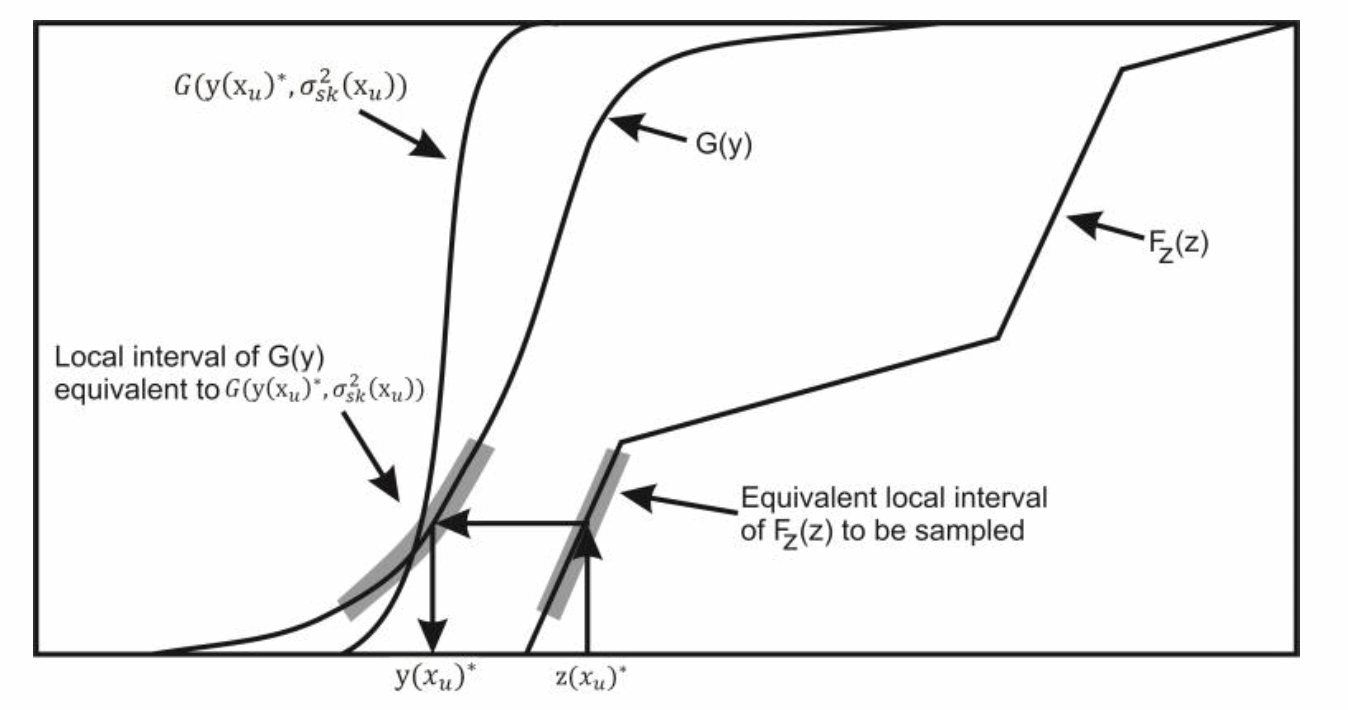
\includegraphics[width=0.5\textwidth]{fig/transfdss}
  \caption{Amostragem global via transformação local feita pela SSD
  \citep{2001amilcarDSS}}
  \label{fig:transfdss}
\end{center}
\end{figure}


Com esta transformação o autor demonstra que é possível amostrar a distribuição
global utilizando amostras de Gaussianas equivalentes a
$G(y(x_u)^*,\sigma^2_{SK}(x_u))$, ou seja, centrada nas médias e com as
variâncias locais da Krigagem. Esta abordagem se diferencia da
\textit{Sequential Gaussian Simulation} (SGS) por não realizar a transformação
da distribuição global para uma variável Gaussiana, o que pode acarretar
problemas em certos casos \citep{2001amilcarDSS}.

O processo de inversão GSI inicia-se sem imagem secundária, efetuando uma SSD
somente utilizando os variogramas e dados de poço. As melhores regiões dos dados
simulados são selecionadas baseado na correlação da sísmica sintética com a
original. Uma imagem auxiliar é então criada com essas melhores regiões e
utilizada como variável secundária na próxima iteração. Os passos da inversão
GSI estão resumidos a seguir:

\begin{enumerate}
  \item Gerar um conjunto de inicial de imagens de impedância acústica
  utilizando SSD
  \item Calcular a sísmica sintética efetuando a convolução das refletividades,
  calculadas a partir das impedâncias, com uma \textit{wavelet} conhecida
  \item Avaliar o casamento das sísmicas sintéticas com a real utilizando
  correlação local
  \item Ordenar as impedâncias por melhor casamento de sua sísmica sintética e
  selecionar delas os melhores traços de impedância. Com os melhores traços,
  compor uma imagem auxiliar para o próximo passo
  \item Gerar um novo conjunto de imagens utilizando co-SSD e retornar ao passo
  2 até que um critério de convergência seja atingido
\end{enumerate}



Uma limitação dos métodos geoestatísticos é a necessidade de transformar o
espaço físico para um espaço deposicional, ou seja, levar em consideração que ao
longo do tempo a estrutura em que foram depositados os sedimentos foi deformada
por falhas e dobramentos. No espaço físico são modelados os processos de
propagação de ondas e fluxo, por exemplo. No espaço deposicional são modeladas
as propriedades das rochas. Para contornar essa limitação é feita uma
transformação onde são utilizados dados chamados de horizontes, criados pelo
especialista para acompanhar as deformações sofridas pelas camadas utilizando
uma superfície interpretada na sísmica. Desta forma assume-se que quando as
camadas de sedimentos foram depositadas elas eram planas e os dados são
transformados horizontalizando as superfícies \citep[p. 140]{caers2011modeling}.
O processo é ilustrado na Figura \ref{fig:hor}. A transformação deve ser
aplicada aos dados de poços e à variável secundária antes de modelar os
variogramas e efetuar a SSD, e revertida para visualizar os resultados e
calcular a sísmica sintética (Equações \ref{eq:refletDiscreta} e
\ref{eq:sismDiscreta}). Esta transformação também é chamada de conversão para
grade estratigráfica.


\begin{figure}[htp]
\begin{center}
  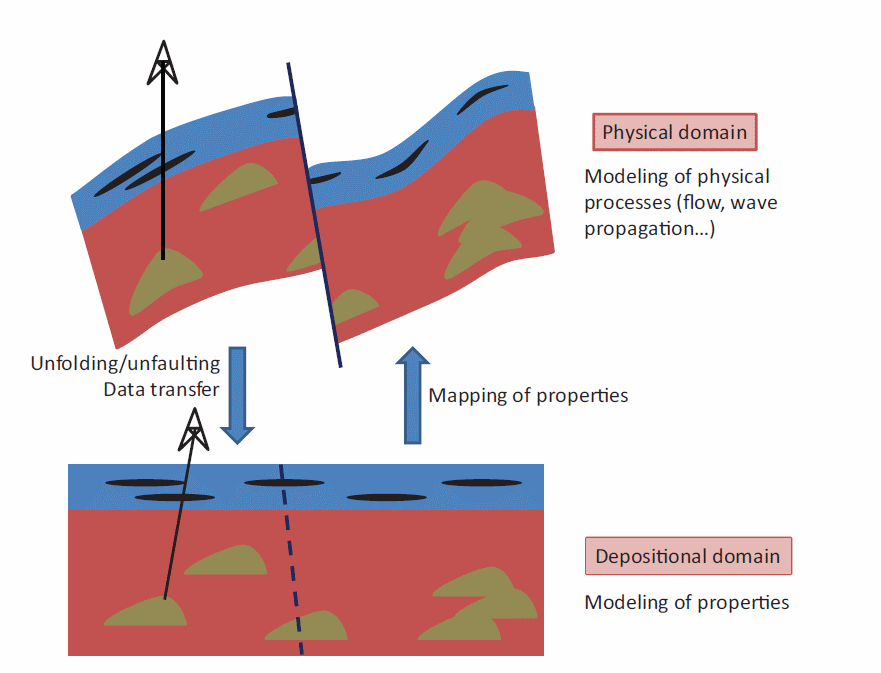
\includegraphics[width=0.6\textwidth]{fig/horizontes}
  \caption{Processo de horizontalização \citep[p. 143]{caers2011modeling}}
  \label{fig:hor}
\end{center}
\end{figure}

\section{Resumo}

Neste capítulo foi revisado o estado da arte em inversão sísmica acústica
com modelagem de incerteza. Pontos críticos dos métodos foram considerados e
identificados para pesquisa futura. O próximo capítulo irá definir a proposta de
pesquisa, apresentar o plano de trabalho e concluir com as perspectivas de
contribuição.





